%----------------------- Преамбула -----------------------
\documentclass[ut8x, 14pt, oneside, a4paper]{extarticle}

\usepackage{extsizes} % Для добавления в параметры класса документа 14pt

% Для работы с несколькими языками и шрифтом Times New Roman по-умолчанию
\usepackage[english,russian]{babel}


% ГОСТовские настройки для полей и абзацев
\usepackage[left=30mm,right=10mm,top=20mm,bottom=20mm]{geometry}
\usepackage{misccorr}
\usepackage{indentfirst}
\usepackage{enumitem}
\setlength{\parindent}{1.25cm}
%\setlength{\parskip}{1em} % поменять
%\linespread{1.3}
\renewcommand{\baselinestretch}{1.5}
\setlist{nolistsep} % Отсутствие отступов между элементами \enumerate и \itemize

% Дополнительное окружения для подписей
\usepackage{array}
\newenvironment{signstabular}[1][1]{
	\renewcommand*{\arraystretch}{#1}
	\tabular
}{
	\endtabular
}

\newcommand{\specsection}[1]{
    \section*{\centering#1}
    \addcontentsline{toc}{section}{#1}
}

% Переопределение стандартных \section, \subsection, \subsubsection по ГОСТу;
% Переопределение их отступов до и после для 1.5 интервала во всем документе
\usepackage{titlesec}



\titleformat{\section}[block]
{\bfseries\normalsize\filcenter}{\thesection}{1em}{}

\titleformat{\subsection}[hang]
{\bfseries\normalsize}{\thesubsection}{1em}{}
\titlespacing\subsection{\parindent}{\parskip}{\parskip}

\titleformat{\subsubsection}[hang]
{\bfseries\normalsize}{\thesubsubsection}{1em}{}
\titlespacing\subsubsection{\parindent}{\parskip}{\parskip}


% Работа с изображениями и таблицами; переопределение названий по ГОСТу
\usepackage{caption}
\captionsetup[figure]{name={Рисунок},labelsep=endash}
\captionsetup[table]{singlelinecheck=false, labelsep=endash}

\usepackage{graphicx}
\usepackage{slashbox} % Диагональное разделение первой ячейки в таблицах

% Цвета для гиперссылок и листингов
\usepackage{color}

% Гиперссылки \toc с кликабельностью
\usepackage{hyperref}

\hypersetup{
	linktoc=all,
	linkcolor=black,
	colorlinks=true,
	urlcolor=black,
}



\usepackage{color} % Цвета для гиперссылок и листингов
%\definecolor{comment}{rgb}{0,0.5,0}
%\definecolor{plain}{rgb}{0.2,0.2,0.2}
%\definecolor{string}{rgb}{0.91,0.45,0.32}
%\hypersetup{citecolor=blue}
\hypersetup{citecolor=black}

\usepackage{listings, listings-rust}
\usepackage{xcolor}
\lstdefinestyle{rustlang}{
    language=Rust,
    backgroundcolor=\color{white},
    basicstyle=\footnotesize\ttfamily,
%    keywordstyle=\color{purple},
%    stringstyle=\color{green},
%    commentstyle=\color{gray},
    numbers=left,
    stepnumber=1,
    numbersep=5pt,
    frame=single,
    tabsize=4,
    captionpos=t,
    breaklines=true,
    breakatwhitespace=true,
    escapeinside={\#*}{*)},
%    morecomment=[l][\color{magenta}]{\#},
    columns=fullflexible
}
\lstset{
	language=rust, % выбор языка для подсветки
	basicstyle=\footnotesize\ttfamily,
	%numberstyle=, % размер шрифта для номеров строк
	stepnumber=1, % размер шага между двумя номерами строк
	numbersep=5pt, % как далеко отстоят номера строк от подсвечиваемого кода
	frame=single, % рисовать рамку вокруг кода
	tabsize=2, % размер табуляции по умолчанию равен 4 пробелам
	captionpos=t, % позиция заголовка вверху [t] или внизу [b]
	breaklines=true,
	breakatwhitespace=true, % переносить строки только если есть пробел
	backgroundcolor=\color{white},
	keywordstyle=\color{blue}
}


\usepackage{ulem} % Нормальное нижнее подчеркивание
\usepackage{hhline} % Двойная горизонтальная линия в таблицах
\usepackage[figure,table]{totalcount} % Подсчет изображений, таблиц
\usepackage{rotating} % Поворот изображения вместе с названием
\usepackage{lastpage} % Для подсчета числа страниц



\usepackage{color}


\usepackage{titlesec}
\usepackage{hyperref}

\titleclass{\subsubsubsection}{straight}[\subsection]

\newcounter{subsubsubsection}[subsubsection]
\renewcommand\thesubsubsubsection{\thesubsubsection.\arabic{subsubsubsection}}
\renewcommand\theparagraph{\thesubsubsubsection.\arabic{paragraph}} % optional; useful if paragraphs are to be numbered

\titleformat{\subsubsubsection}
{\normalfont\normalsize\bfseries}{\thesubsubsubsection}{1em}{}
\titlespacing*{\subsubsubsection}
{14mm}{3.25ex plus 1ex minus .2ex}{1.5ex plus .2ex}

\makeatletter
\renewcommand\paragraph{\@startsection{paragraph}{5}{\z@}%
	{3.25ex \@plus1ex \@minus.2ex}%
	{-1em}%
	{\normalfont\normalsize\bfseries}}
\renewcommand\subparagraph{\@startsection{subparagraph}{6}{\parindent}%
	{3.25ex \@plus1ex \@minus .2ex}%
	{-1em}%
	{\normalfont\normalsize\bfseries}}
\def\toclevel@subsubsubsection{4}
\def\toclevel@paragraph{5}
\def\toclevel@paragraph{6}
\def\l@subsubsubsection{\@dottedtocline{4}{7em}{4em}}
\def\l@paragraph{\@dottedtocline{5}{10em}{5em}}
\def\l@subparagraph{\@dottedtocline{6}{14em}{6em}}
\makeatother

\setcounter{secnumdepth}{4}
\setcounter{tocdepth}{4}

\usepackage{xcolor}
\usepackage{listings}

\usepackage{xparse}


\NewDocumentCommand{\codeword}{v}{%
	\texttt{\textcolor{black}{#1}}%
}

\lstset{language=C,keywordstyle={\bfseries \color{black}}}
\captionsetup{labelsep=endash}
\usepackage[final]{pdfpages}

\usepackage{placeins}
\usepackage{listings}
\usepackage{longtable}
\usepackage{tikz}


\usepackage{pgfplots}
\usepackage{totcount}
\newtotcounter{citnum} %From the package documentation

\makeatletter
\renewcommand\@biblabel[1]{#1.}
\makeatother

\newcommand{\img}[3] {
    \begin{figure}[h]
        \center{\includegraphics[height=#1]{inc/img/#2}}
        \caption{#3}
        \label{img:#2}
    \end{figure}
}
\newcommand{\boximg}[3] {
    \begin{figure}[h]
        \center{\fbox{\includegraphics[height=#1]{inc/img/#2}}}
        \caption{#3}
        \label{img:#2}
    \end{figure}
}

\renewcommand{\labelenumi}{\arabic{enumi}.}
\renewcommand{\labelenumii}{\arabic{enumi}.\arabic{enumii}.}
\renewcommand{\labelenumiii}{\arabic{enumi}.\arabic{enumii}.\arabic{enumiii}.}
\renewcommand{\labelenumiv}{\arabic{enumi}.\arabic{enumii}.\arabic{enumiii}.\arabic{enumiv}.}


\begin{document}

\pagenumbering{gobble}

    \normalsize

    \pagenumbering{arabic}
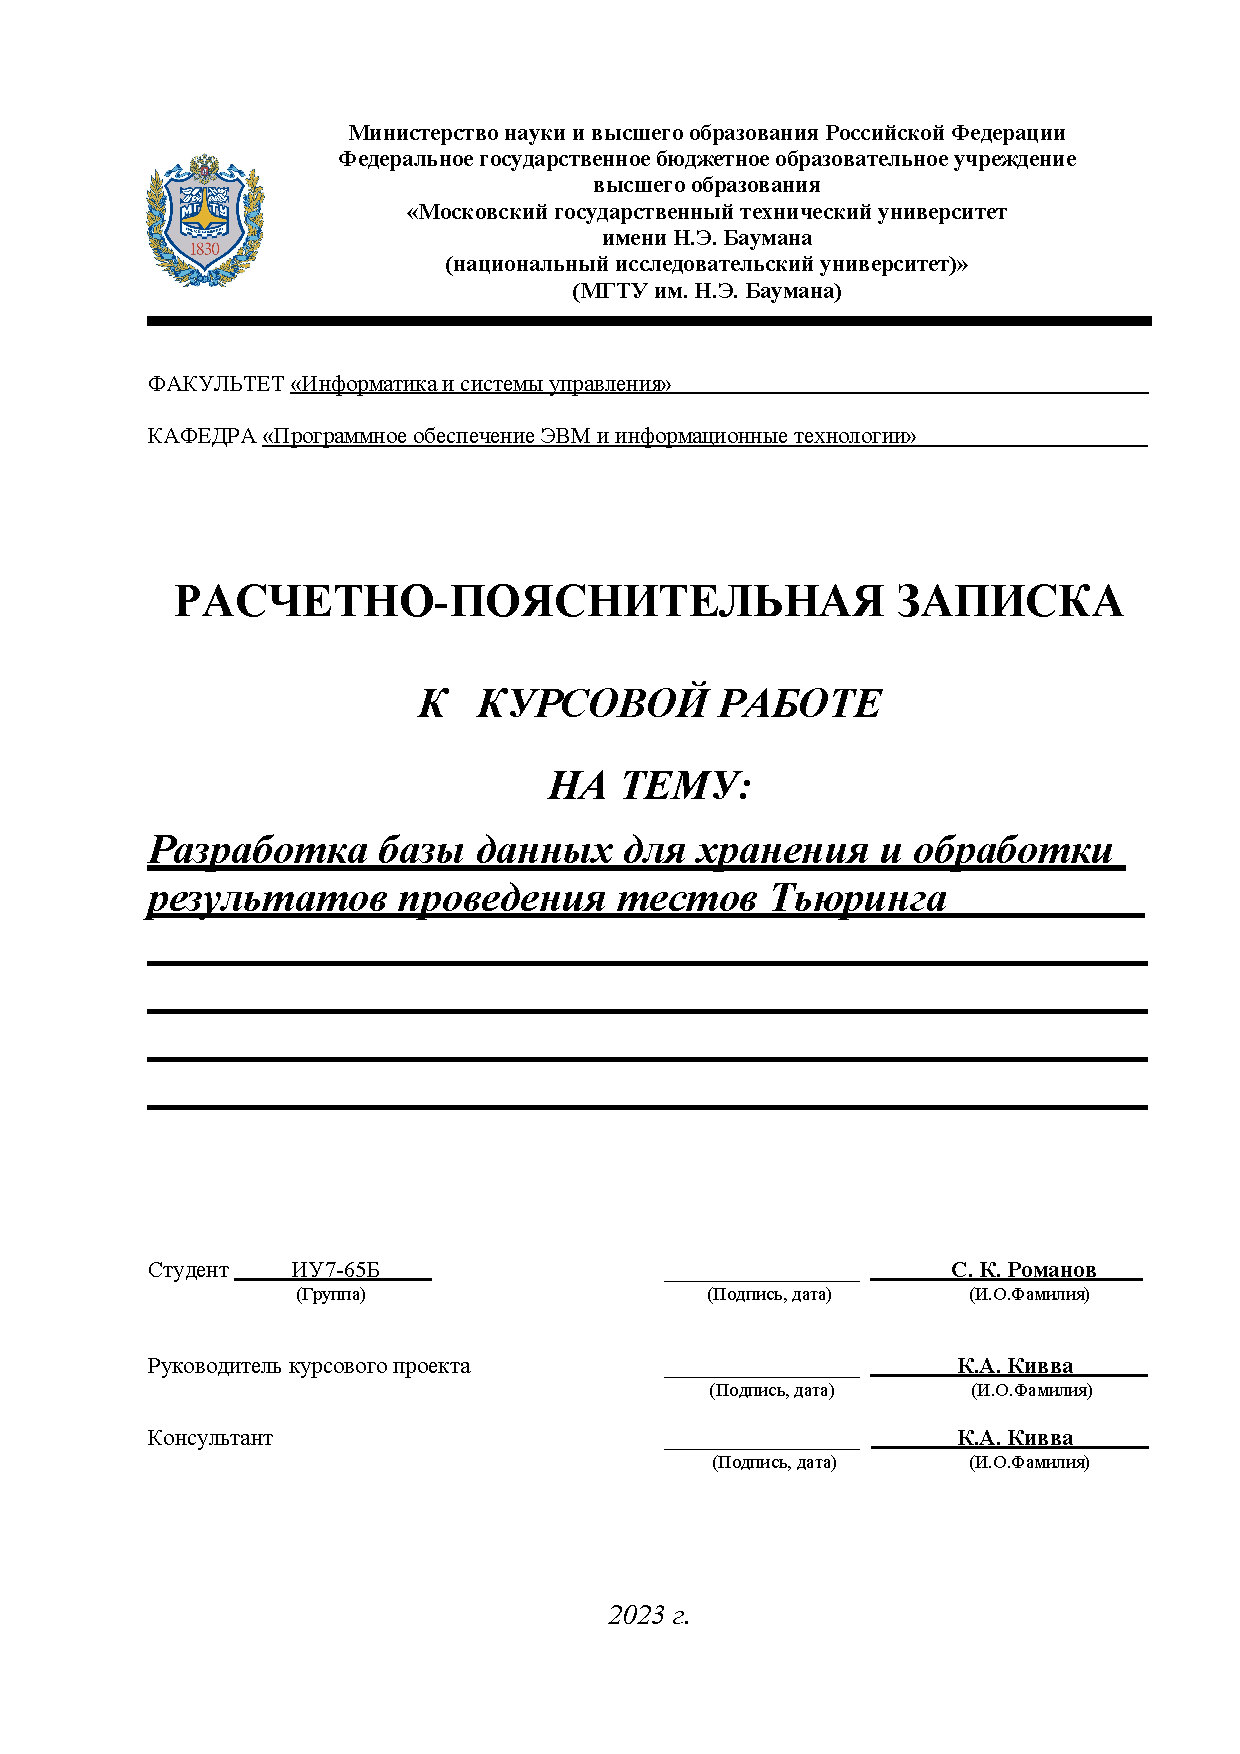
\includepdf[pages={1}]{RPZ_title.pdf}

\specsection{РЕФЕРАТ}

Расчётно-пояснительная записка содержит 59 с., 16 рис., 3 табл., 31 ист.

Цель работы: создание базы данных для хранения результатов тестов Тьюринга.

Ключевые слова: базы данных, SurrealDB, граф, отношения.

В данной работе проводится изучение принципов работы баз данных.

Объектом исследования является модель представления результатов тестов Тьюринга в виде графа.

Результаты: разработана программа, предназначенная для работы с базами данных. Проанализированы разные системы управления базами данных.

\pagebreak

\newpage
\renewcommand{\contentsname}{\normalsize\bfseries\centering СОДЕРЖАНИЕ}
    \tableofcontents
    \normalsize

\specsection{ОПРЕДЕЛЕНИЯ}
% \addcontentsline{toc}{specsection}{ОПРЕДЕЛЕНИЯ}

В настоящей расчетно-пояснительной записке применяют следующие термины с соответствующими определениями.\\

\begin{description}
	\item{Natural Language Processing} --- <<Обработка текстов на естественном языке>> относится к области компьютерных наук, а точнее к области искусственного интеллекта или ИИ, связанной с предоставлением компьютерам возможность понимать текст и произносимые слова почти так же, как люди.
   НЛП сочетает в себе вычислительную лингвистику — моделирование человеческого языка на основе правил — со статистическими моделями, машинным обучением и моделями глубокого обучения. Вместе эти технологии позволяют компьютерам обрабатывать человеческий язык в виде текстовых или голосовых данных и «понимать» его полное значение, включая намерения и чувства говорящего или пишущего.~\cite{nlp}
	\item{ACID} --- В контексте обработки транзакций аббревиатура ACID относится к четырем ключевым свойствам транзакции: атомарность (Atomicity), непротиворечивость (Consistency), изоляция (Isolation) и устойчивость (Durability).~\cite{gdb-def}.
	\item{Graph Database} --- база данных, использующая структуры графов для семантических запросов с узлами, ребрами и свойствами для представления и хранения данных.~\cite{gdb-def}. 
\end{description}

\specsection{ОБОЗНАЧЕНИЯ И СОКРАЩЕНИЯ}
% \addcontentsline{toc}{specsection}{ОБОЗНАЧЕНИЯ И СОКРАЩЕНИЯ}

В настоящей расчетно-пояснительной записке применяют следующие сокращения и обозначения.\\

\begin{description}	
	\item{NLP} --- <<Natural Language Processing>>.
	\item{ACID} --- <<Atomicity, Consistency, Isolation, Durability>>.
	\item{SQL} --- <<Structured Query Language>>.
	\item{GDB} --- <<Graph Database>>
	\item{ИИ} --- <<Искусственный Интеллект>>
	\item{UUID} --- <<Universally Unique IDentifier>>
\end{description}


\specsection{ВВЕДЕНИЕ}
% \addcontentsline{toc}{specsection}{Введение}

Тест Тьюринга --- это способ определения способности машины производить интеллектуальные действия, неотличимые от действий человека. В современном мире тесты Тьюринга стали одним из ключевых инструментов для определения искусственного интеллекта. Эти тесты позволяют определить, насколько хорошо компьютер может имитировать разговор человека.
Для проведения теста Тьюринга используется программное обеспечение, которое имитирует человеческое поведение и должно убедить эксперта в том, что он общается с живым человеком. Результаты проведения тестов могут быть использованы для разработки и улучшения алгоритмов искусственного интеллекта. Это позволяет разработчикам алгоритмов искусственного интеллекта улучшать свои продукты и технологии.

Примерами таких алгоритмов являются алгоритмы обработки естественных языков (Natural Language Processing --- NLP). В общих словах --- это совокупность методов и техник, которые позволяют компьютерам анализировать, понимать и генерировать естественный язык. NLP используется в ряде приложений, включая автоматический перевод, распознавание речи и анализ текста. Анализ результатов тестирования поможет в будущем улучшить данные модели, позволяя избегать различные грамматические, орфографические и смысловые ошибки. 

Модели от команды OpenAI и многие другие играют важную роль в развитии искусственного интеллекта. GPT-3 неплохо справляется с созданием художественной литературы, поэзии, пресс-релизов, кода, музыки, шуток, технических руководств и новостных статей. Возможно, как предполагает Чалмерс (2020, Other Internet Resources), GPT-3 «предлагает потенциальный бездумный путь к общему искусственному интеллекту». Но, конечно, GPT-3 даже не близок к прохождению теста Тьюринга: на глобальном уровне — учитывая значения нескольких предложений, абзацев или двустороннего диалога — становится очевидным, что GPT-3 не понимает, о чем говорит. У него нет здравого смысла (Common Sense) или способности отслеживать объекты во время обсуждения. Разработанная база данных для хранения и обработки результатов тестов Тьюринга --- это хороший инструмент для создания более развитых систем искусственного интеллекта. 

Цель данной работы --- разработать базу данных для хранения результатов проведения тестов Тьюринга. База данных должна содержать информацию о тестируемых программах, экспертах, результатах проведения тестов и другие данные, необходимые для анализа результатов.

Чтобы достигнуть поставленной цели, требуется решить следующие задачи: 
\begin{itemize}
    \item[$-$] Определить структуру базы данных и ее таблиц.
    \item[$-$] Разработать модели данных для каждой таблицы.
    \item[$-$] Написать запросы для вставки, обновления и удаления данных в таблицах.
    \item[$-$] Реализовать функционал для получения результатов проведенных тестов, с возможностью фильтрации и сортировки по различным полям.
    \item[$-$] Разработать интерфейс пользователя для удобного использования базы данных. 
\end{itemize}

\section{Аналитический раздел}

В данном разделе описана структура теста Тьюринга.  
Представлен анализ способов хранения данных и систем управления базами данных. 

\subsection{Анализ предметной области}
Тест Тьюринга --- это простой метод определения того, может ли машина продемонстрировать человеческий интеллект~\cite{turing-def}.
На рисунке~\ref{img:turing} представлено схематическое изображение этого метода.

\img{100mm}
{turing}
{Тест Тьюринга}

Тьюринг в своей работе~\cite{10.1093/mind/LIX.236.433} описывает следующий вид игры.
Пусть есть человек, машина и эксперт.
Эксперт находится в комнате, отделенной от другого человека и машины. 
Цель игры состоит в том, чтобы эксперт определил, кто из двух является человеком, а кто машиной. 
Эксперт знает человека и машину по меткам <<X>> и <<Y>> --- но, по крайней мере в начале игры, не знает, кто из них человек и кто -- машина --- и в конце игры он должен сказать либо «X --- это человек, а Y --- машина», либо «X --- это машина, а Y --- человек».
Эксперту разрешается задавать человеку и машине вопросы следующего вида: <<Скажите, пожалуйста, X, играет ли X в шахматы?>> Кто бы из машины и другого человека ни был X, он должен отвечать на вопросы, адресованные X.
Цель машины состоит в том, чтобы попытаться заставить эксперта ошибочно заключить, что машина --- это другой человек; цель другого человека состоит в том, чтобы попытаться помочь эксперту правильно идентифицировать машину~\cite{sep-turing-test}.

% Следует отметить, что во времена Тьюринга, было ограничение, что ответы поступали через ограниченные врменные рамки, поскольку время ответа компьютера было гораздо больше, чем у человека. 
% Сегодня это ограничение сохраняется, однако из-за обратного: реакция компьютера быстрее, чем реакция человека~\cite{10.1093/mind/LIX.236.433}.

\subsection{Формализация данных}

Для решения задачи хранения теста Тьюринга необходимо хранить следующие данные:
\begin{enumerate}
  \item Данные о человеке, машине и эксперте;
  \begin{enumerate}
    \item Для человека:
      \begin{itemize}
        \item[$-$] Имя;
        \item[$-$] Пол;
        \item[$-$] Возраст;
        \item[$-$] Национальность.
      \end{itemize}
    \item Для машины:
      \begin{itemize}
        \item[$-$] Модель Искусственного Интеллекта;
        \item[$-$] Разработчик модели.
      \end{itemize}
    \item Для эксперта:
      \begin{itemize}
        \item[$-$] Имя;
        \item[$-$] Пол;
        \item[$-$] Возраст;
        \item[$-$] Национальность.
      \end{itemize}
  \end{enumerate}
  \item Данные о заданных вопросах и полученных ответах, а также вердикт эксперта c предположением о сущностях ответчиков;
    \begin{itemize}
      \item[$-$] Для вопросов --- текст вопроса.
      \item[$-$] Для ответов --- текст ответа.
      \item[$-$] Для вердикта --- корректность вердикта.
    \end{itemize}
  \item Данные об отдельном эксперименте:
    \begin{itemize}
      \item[$-$] Длительность проведения эксперимента;
      \item[$-$] Время, отведенное на дачу ответов субъектами.
    \end{itemize}
  \item Данные, о связях между сущностями:
    \begin{itemize}
      \item[$-$] Последовательность вопросов - ответов, оканчивающаяся вердиктом;
      \item[$-$] Связь между ответом и теми, кто его дал;
      \item[$-$] Связь между вопросом и теми, кто его задал;
      \item[$-$] Связь между вердиктом, тем кто его задал, и относительно каких субъектов он был вынесен;
      \item[$-$] Связь между экспериментом и всеми сущностями включенными в данный эксперимент.
    \end{itemize}
\end{enumerate}

На рис.~\ref{img:chen} изображена ER-диаграмма предметной области.

\img{200mm}
{chen}
{ER-диаграмма предметной области}

\clearpage

\subsection{Способы хранения данных}

Поскольку в конце теста выносится вердикт о том, является ли отвечающий машиной или человеком, необходимо также хранить, какие ответы были даны, в каком порядке и каким актором. 
Эти данные должны быть доступны для обработки и сравнения в процессе игры.
 
Один из способов хранения данных --- это использование реляционных баз данных. В этом случае можно создать таблицы для каждого объекта (люди, машины и эксперты, вопросы и ответы, и т.д.) и связать их отношениями. 
Например, таблицы <<Person>>, <<Computer>> и <<Interrogator>> могут быть связаны через внешние ключи. 
Это является надежным и проверенным способом хранения данных.

Однако более эффективный способ хранения сильносвязанных данных --- это использование графовых баз данных (GDB), таких как \texttt{SurrealDB} или \texttt{Neo4j}~\cite{DBLP:journals/corr/LinMPS16}. 
В этом случае каждый объект может быть представлен узлом графа, а отношения между объектами --- ребрами графа. Схематическое изображение графовой модели данных можно увидеть на рисунке~\ref{img:graph_new}.

\img{100mm}
{graph_new}
{Представление базы данных в виде графа}

Ключевым понятием такой базы данных является граф (или ребро, или взаимосвязь).
Граф связывает элементы данных в хранилище с набором узлов и ребер, причем ребра представляют отношения между узлами. 
Отношения позволяют напрямую связывать данные в хранилище и во многих случаях извлекать их с помощью одной операции. 
Графовые базы данных удерживают отношения между данными в качестве приоритета.
Запросы по отношениям проходят быстро, потому что они постоянно хранятся в базе данных в качестве отдельных сущностей.
Отношения можно визуализировать с помощью графов, что делает их полезными для сильно взаимосвязанных данных~\cite{graph-exp}.
В графовых базах данных нет необходимости использовать сложные \texttt{JOIN}-запросы, что может существенно упростить запросы к данным по отношениям.

Графовые базы данных также обеспечивают быстрый доступ к данным по отношениям, что делает их эффективными при работе с глубоко связанными данными. Они также позволяют легко добавлять новые данные в граф без необходимости изменения схемы базы данных.
Однако, реляционные базы данных обладают более высокой надежностью и могут обеспечивать лучшую производительность при выполнении сложных запросов, особенно если используются правильно настроенные индексы.

Таким образом, выбор между реляционными базами данных и графовыми зависит от конкретных требований проекта.
В контексте данной работы, графовая модель подходит больше, чем реляционная, потому что тест Тьюринга включает в себя множество связей между объектами (человек, машина, эксперт, вопросы и ответы и т.д.), которые можно представить в виде графа.

Графовая модель также становится еще более привлекательной, если вспомнить какая идея была обозначена в начале данной работы: создание инструмента для улучшения искусственного интеллекта.
Результаты тестов Тьюринга, которые будут храниться в графовой базе данных, можно будет использовать для эффективного, по сравнению с традиционными реляционными базами данных, обучения ИИ. 
Эффективность достигается за счет того, что данные, используемые для обучения ИИ, представлены в виде графа, а не в виде стандартных <<табличных>> значений~\cite{besta2022neural}. 
Таким образом, схожая структура данных внутри БД поможет разработать более гибкую и быстродействующую систему при меньших затраченных ресурсах.

На рис.~\ref{img:graph-bench} можно увидеть результаты сравнения 3 различных баз данных: реляционной (\texttt{PostgreSQL}), графовой (\texttt{Neo4j}) и мультимодельной (\texttt{ArangoDB}). 
Исходя из графика видно, что графовая, а также мультимодельная база данных обеспечивает лучшую производительность при выполнении запросов по отношениям (\texttt{JOIN}-запросов), а также \texttt{PROJECTION}-запросов. 
Скорость графовой и мультимодельной баз данных относительно реляционной по \texttt{PROJECTION}-запросам объясняется особенностью \texttt{key-value} хранилищ, лежащих в основе графовой и мультимодельной баз данных.
При этом, реляционная база данных обеспечивает лучшую производительность при выполнении операций, не связанных с отношениями, а именно \texttt{ORDER BY} и \texttt{AGGREGATION}.

\clearpage

\img{100mm}
{graph-bench}
{Сравнение времени выполнения атомарных операций над различными базами данных.}

\subsection{Ролевая модель}
В системе определены четыре возможные роли, ограничивающие доступ к получению/добавлению информации.
\begin{enumerate}
  \item Эксперт --- пользователь, обладающий возможностью задавать новые вопросы подопытным, а также выносить вердикт на оснвое полученных решений, имеет доступ к прочтению всех данных в рамках сессии;
  \item Компьютер --- пользователь, обладающий возможностью дачи ответов на вопросы эксперта, имеет доступ к чтению своих прошлых ответов и вопросов к ним в рамках сессии;
  \item Человек --- пользователь, обладающий равными с комьютером правами и воможностями. Ввиду различия характеристик между человеком и компьютером, в системе необходимо отдельно хранить данные об этих сущностях, а также выделить отдельные роли;
  \item Администратор --- пользователь, обладающий возможностью добавления/удаления/изменения всех пользователей, сущностей и полей базы данных, а также просмотра всех данных в рамках базы данных.
\end{enumerate}

На рисунке~\ref{img:roles} представлена диаграмма ролей.

\img{160mm}
{roles}
{Диаграмма ролей}

% \clearpage

\subsection{Системы управления базами данных}

% Для выбора системы управления базами данных необходимо учитывать требования к производительности и масштабируемости приложения.
%
% Реляционные базы данных имеют высокую надежность и поддерживают ACID-свойства транзакций. Они также обеспечивают хорошую производительность при выполнении сложных запросов. Однако, они требуют дополнительного управления индексами и ключевыми полями.
%
% Графовые базы данных обеспечивают высокую производительность при работе с глубоко связанными данными.
% Граф связывает элементы данных в хранилище с набором узлов и ребер, причем сами ребра представляют отношения между узлами.
% Отношения позволяют напрямую связывать данные в хранилище и во многих случаях извлекать их с помощью одной операции.
% Отношения между данными в подобных системах имеют приоритет над самими данными, поэтому запрос по отношениям является крайне быстрой операцией, поскольку они постоянно хранятся в базе данных. 
% Также отношения можно визуализировать с помощью графов, что делает их полезными для сильно взаимосвязанных данных. 

\subsubsection{SurrealDB}

\texttt{SurrealDB} --- мультимодельная \texttt{NewSQL} база данных, которая работает в режиме полной схемы (\texttt{SCHEMAFULL}) или без схемы (\texttt{SCHEMALESS}), с таблицами, ссылками на записи между документами (без \texttt{JOIN}) и функциями моделирования базы данных на основе графов~\cite{surrealdb}.

Благодаря использованию \texttt{SurrealDB} особых методов сегментирования и репликации, становится возможным повысить производительность за счет распределения нагрузки между несколькими компьютерами~\cite{surrealarch}.

Также особая архитектура базы данных позволяет работать как в оперативной памяти (\texttt{in-memory}), на дисковом пространстве (\texttt{on-disk}) или как распределенная база данных, используя \texttt{TiKV}~\cite{tikv}.

Поскольку \texttt{SurrealDB} --- мультимодельная база данных, становятся также возможными классические реляционные методики проектирования баз данных, что повышает гибкость итоговой системы.

\subsubsection{Neo4j}

\texttt{Neo4j} --- это графовая база данных, которая позволяет хранить, управлять и анализировать связанные данные. 
Она была разработана с учетом графовой модели данных, в которой данные представлены в виде узлов (вершин) и связей (ребер)~\cite{neo4j}. 

Одним из преимуществ \texttt{Neo4j} является то, что она позволяет эффективно моделировать и анализировать сложные связи между данными, такие как в социальных сетях, географических картах и сетях предприятий.
Это делает ее очень полезной для приложений, которые требуют быстрого доступа к сложным связным данным и быстрой обработки запросов.

Однако поскольку \texttt{Neo4j} --- исключительно графовая база данных, хранение и получение данных без каких-либо связей друг с другом может вызвать проблемы с производительностью, вне зависимости от размера запроса~\cite{neocons}.

\subsection{ArangoDB}

Подобно \texttt{SurrealDB}, \texttt{ArangoDB} также является мультимодельной базой даных, однако при этом является \texttt{NoSQL} базой данных в противовес \texttt{NewSQL}.

\texttt{ArangoDB} ---  был разработан специально для обслуживания различных типов баз данных \texttt{NoSQL}. 
Таким образом, варианты использования ArangoDB могут включать одновременную разработку баз данных, ориентированных на ключ, граф или документ~\cite{arangodb}.

Отличительной чертой всех \texttt{NoSQL} баз данных является отсутствие возможности объявления схемы данных внутри таблицы, и \texttt{ArangoDB} не исключение. 
Несмотря на то, что у \texttt{ArangoDB} есть внешний инструмент валидации данных через \texttt{JSON}-схемы, данная возможность проигрывает в гибкости настройки полноценным схемам традиционных реляционных и \texttt{NewSQL} баз данных.
Для непосредственного сравнения, документация \texttt{SurrealDB}~\cite{surrealdb-doc} насчитывает порядка 30 базовых типов, спецификация \texttt{JSON}-схемы~\cite{json-type} насчитывает всего лишь 7.
\subsection{Выбор СУБД для решения задачи}

Среди графовых баз данных можно выделить три наиболее подходящие системы: \texttt{SurrealDB}, \texttt{Neo4j} и \texttt{ArangoDB}.
Эти три СУБД обеспечивают быстрый доступ к данным по отношениям, что делает их эффективными при работе с глубоко связанными данными.

Однако \texttt{SurrealDB} имеет дополнительные преимущества перед \texttt{Neo4j} и \texttt{ArangoDB}. 
В противовес \texttt{Neo4j}, она является мультимодельной базой данных, что позволяет эффективное хранение и получение несвязанных данных, например выгрузка всех экспертов, которые учавстовали в различных экспериментах.
В таких случаях, \texttt{Neo4j} может испытывать определенные проблемы связанные в первую очередь с производительностью.

Если сравнивать \texttt{SurrealDB} c \texttt{ArangoDB}, то \texttt{SurrealDB} предоставляет более гибкий инструмент настройки схемы базы данных.

\subsection*{Вывод}

В данном разделе:
\begin{itemize}
  \item[$-$] рассмотрена сущность и структура теста Тьюринга;
  \item[$-$] определены ключевые роли в рамках эксперимента, связанного с тестом Тьюринга;
  \item[$-$] проанализированы способы хранения информации для системы и выбраны оптимальные способы для решения поставленной задачи;
  \item[$-$] были рассмотрены два различных типа баз данных: реляционные и графовые;
  \item[$-$] было выявлено, что для решения задачи теста Тьюринга наиболее подходящей является графовая база данных, а конкретно \texttt{SurrealDB}.
\end{itemize}


\section{Конструкторский раздел}
В данном разделе представлены этапы проектирования выделенных в предыдущем разделе базы данных, нужной для решения задачи.

\subsection{Проектирование базы данных для хранения Тестов Тьюринга}  
База данных для хранения Тестов Тьюринга будет реализована с использованием СУБД SurrealDB.
В базе данных будет существовать 7 таблиц и 7 типов отношений. 
Схема разработанной базы данных представлена на рисунке~\ref{img:er_new}.

\img{125mm}
{er_new}
{Схема разработанной базы данных.}

Поля таблицы \texttt{Interrogator}: 
\begin{enumerate}
    \item \texttt{UniqueID} --- уникальный идентификатор --- \texttt{UUID};
    \item \texttt{Name} --- имя <<эксперта>> --- строка;
    \item \texttt{Gender} --- пол <<эксперта>> --- строка;
    \item \texttt{Age} --- возраст <<эксперта>> --- целое число;
    \item \texttt{Nationality} --- национальность <<эксперта>> --- строка.
\end{enumerate}

Данная таблица отвечает за хранение данных, связанных с экспертом, проводящим эксперимент.
Эта таблица связана со следующими таблицами:
\begin{itemize}
    \item[$-$] \texttt{Session} --- через отношение \texttt{:ParticipateIn};
    \item[$-$] \texttt{Answer} --- через отношение \texttt{:Asks};
    \item[$-$] \texttt{Verdict} --- через отношение \texttt{:Gives}.
\end{itemize}

Поля таблицы \texttt{Computer}:
\begin{enumerate}
    \item \texttt{UniqueID} --- уникальный идентификатор --- \texttt{UUID};
    \item \texttt{Model} --- Модель ИИ, проходившая тест --- строка;
    \item \texttt{DevelopedBy} --- Разработчики указанной модели ИИ --- строка.
\end{enumerate}

Данная таблица отвечает за хранение данных, связанных с компьютером, участвующем в эксперименте. 
Эта таблица связана со следующими таблицами:
\begin{itemize}
    \item[$-$] \texttt{Session} --- через отношение \texttt{:ParticipateIn};
    \item[$-$] \texttt{Answer} --- через отношение \texttt{:Gives};
    \item[$-$] \texttt{Verdict}. --- через отношение \texttt{:Mentions}.
\end{itemize}

Поля таблицы \texttt{Human}:
\begin{enumerate}
    \item \texttt{UniqueID} --- уникальный идентификатор --- \texttt{UUID};  
    \item \texttt{Name} --- имя человека --- строка;
    \item \texttt{Gender} --- пол человека --- строка;
    \item \texttt{Age} --- возраст человека --- строка; 
    \item \texttt{Nationality} --- национальность человека --- строка.
\end{enumerate}

Данная таблица отвечает за хранение данных, связанных с человеком, участвующем в эксперименте. 
Эта таблица связана со следующими таблицами:
\begin{itemize}
    \item[$-$] \texttt{Session} --- через отношение \texttt{:ParticipateIn};
    \item[$-$] \texttt{Answer} --- через отношение \texttt{:Gives};
    \item[$-$] \texttt{Verdict} --- через отношение \texttt{:Mentions}.
\end{itemize}

Поля таблицы \texttt{Answer}:
\begin{enumerate}
    \item \texttt{ItemID} --- уникальный идентификатор --- \texttt{UUID}.
    \item \texttt{AnswerText} --- текст ответа --- строка.
\end{enumerate}

Данная таблица отвечает за хранение данных, связанных с ответами, данными в эксперименте. 
Следует отметить, что ответы, данные на протяжении всех экспериментов, являются уникальными сущностями, или, иными словами, в базе данных нет двух одинаковых ответов на любой из вопросов.
Данная особенность преследует цель показать связь между вопросами и ответами, и как различные вопросы могут привести к одним и тем же ответам, либо же, как компьютер и человек в экперименте могут дать одинаковый ответ.

Эта таблица связана со следующими таблицами:
\begin{itemize}
    \item[$-$] \texttt{Session} --- через отношение \texttt{:Includes};
    \item[$-$] \texttt{Answer} --- через отношения \texttt{:AnsweredBy} и \texttt{:Follows};
    \item[$-$] \texttt{Computer} --- через отношение \texttt{:Gives};
    \item[$-$] \texttt{Human} --- через отношение \texttt{:Gives};
    \item[$-$] \texttt{Verdict} --- через отношение \texttt{:Follows}.
\end{itemize}

Поля таблицы \texttt{Question}:
\begin{enumerate}
    \item \texttt{ItemID} --- уникальный идентификатор --- \texttt{UUID}.
    \item \texttt{QuestionText} --- текст вопроса --- строка.
\end{enumerate}

Данная таблица отвечает за хранение данных, связанных с вопросами, данными в эксперименте экспертом. 
Следует отметить, что вопросы, данные на протяжении всех экспериментов, как и ответы, упомянутые выше, являются уникальными сущностями, или, иными словами, в базе данных нет двух одинаковых вопросов.
Данная особенность преследует цель показать связь между вопросами и ответами, и как на один вопрос можно привести множество различных ответов.

Эта таблица связана со следующими таблицами:
\begin{itemize}
    \item[$-$] \texttt{Session} --- через отношение \texttt{:Includes};
    \item[$-$] \texttt{Answer} --- через отношения \texttt{:AnsweredBy} и \texttt{:Follows};
    \item[$-$] \texttt{Interrogator} --- через отношение \texttt{:Asks}.
\end{itemize}

Поля таблицы \texttt{Verdict}:
\begin{enumerate}
    \item \texttt{ItemID} --- уникальный идентификатор --- \texttt{UUID};
    \item \texttt{Correct} --- Верен ли вердикт, выданный экспертом --- ложь / истина.
\end{enumerate}

Данная таблица отвечает за хранение данных, связанных с вердиктами, данными экспертами по окончанию экспериментов.
После любого данного ответа, эксперт может закончить эксперимент и выдать свой вердикт, кто является компьютером, а кто человеком.

Эта таблица связана со следующими таблицами:
\begin{itemize}
    \item[$-$] \texttt{Session} --- через отношение \texttt{:Includes};
    \item[$-$] \texttt{Answer} --- через отношение \texttt{:Follows};
    \item[$-$] \texttt{Interrogator} --- через отношение \texttt{:Gives};
    \item[$-$] \texttt{Computer} --- через отношение \texttt{:Mentions};
    \item[$-$] \texttt{Human} --- через отношение \texttt{:Mentions}.
\end{itemize}

Поля таблицы \texttt{Session}:
\begin{enumerate}
    \item \texttt{SessionID} --- уникальный идентификатор --- \texttt{UUID};
    \item \texttt{TimeFrame} --- период времени, отведенный на ответ на вопрос --- время;
    \item \texttt{TimeSpent} --- продолжительность сессии --- время.
\end{enumerate}

Данная таблица отвечает за хранение данных, связанных с различными экспериментами.
Данная таблица является свеого рода мета-таблицей, по связи с которой можно получить данные о всех сущностях, участвующих в эксперименте.

Эта таблица связана со следующими таблицами:
\begin{itemize}
    \item[$-$] \texttt{Question} --- через отношение \texttt{:Includes};
    \item[$-$] \texttt{Answer} --- через отношение \texttt{:Includes};
    \item[$-$] \texttt{Answer} --- через отношение \texttt{:Includes};
    \item[$-$] \texttt{Interrogator} --- через отношение \texttt{:ParticipateIn};
    \item[$-$] \texttt{Computer} --- через отношение \texttt{:ParticipateIn};
    \item[$-$] \texttt{Human} --- через отношение \texttt{:ParticipateIn}.
\end{itemize}

Поля рёбер \texttt{:AnsweredBy} и \texttt{:Follows}:
\begin{enumerate}
    \item \texttt{Order} --- порядковый номер вопроса/ответа/вердикта в системе - целое число
\end{enumerate}

% Пример SQL запроса, утилизирующий множественные JOIN-операции: 

Особенность \texttt{SurrealDB} заключается в том, что отношения также могут иметь дополнительные поля, характеризующие их.
Поле \texttt{Order} необходимо для построения контекста ответов/вопросов поскольку ответ может различаться от того, какие ответы были даны ранее.

\subsection{Структура разрабатываемого ПО}
Предполагается, что разрабатываемый проект является одним цельным \texttt{Electron}-подобным~\cite{electron} приложением.
Серверная часть и графический интерфейс упаковывается в единый бинарный файл, предоставляя возможность создать различные версии приложения под различные операционные системы.
В общем смысле, серверная часть коммуницирует с базой данных, доставляя результат к графическому интерфейсу в рамках единого приложения.

Общая схема архитектура приложения представлена на рисунке~\ref{img:arch}

\img{75mm}
{arch}
{Схема архитектуры приложения}


\subsection*{Вывод}
В данном разделе были представлены проектирование базы данных, рассмотрены особенности используемой СУБД на архитектурном уровне и была показана структура разрабатываемого ПО.

\section{Технологический раздел}

В данном разделе представлены 
\begin{itemize}
    \item[$-$] архитектура;
    \item[$-$] средства разработки программного обеспечения;
    \item[$-$] детали реализации;
    \item[$-$] способы взаимодействия с программным продуктом.
\end{itemize}

\subsection{Архитектура}
Предполагается, что разрабатываемый проект является одним цельным Electron-подобным~\cite{electron} приложением.
Серверная часть и графический интерфейс упаковывается в единый бинарный файл, предоставляя возможность создать различные версии приложения под различные операционные системы.
В общем смысле, серверная часть коммуницирует с базой данных, доставляя результат к графическому интерфейсу в рамках единого приложения.

Общая схема архитектура приложения представлена на рисунке~\ref{img:arch}

\img{95mm}
{arch}
{Схема архитектуры приложения}

\subsection{Средства реализации}

Основным языком программирования является мультипарадигменный язык Rust~\cite{rust}.
\begin{itemize}
    \item[$-$] Одно из главных достоинств данного языка это гарантия безопасной работы с памятью при помощи системы
    статической проверки ссылок, так называемый Borrow Checker~\cite{borrow-checker}.
    \item[$-$] Отсутствие сборщика мусора, как следствие, более экономная работа с ресурсами.
    \item[$-$] Встроенный компилятор, постaвляемый совместно с пакетным менеджером Cargo.
    \item[$-$] Кросс-платформенность, от UNIX и MacOS приложений до Web - приложений.
    \item[$-$] \texttt{SurrealDB} и \texttt{Rust} написаны на одном и том же языке, в следствии чего инструментарий наиболее плотно работает с непосредственно самой базой данных.
    \item[$-$] Важно отметить, что язык программирования Rust сопоставим по скорости с такими языками как С и С++,
    предоставляя в то же время более широкий функционал для тестирования кода и контроля памяти.
\end{itemize}

Также в рамках языка \texttt{Rust} был выбран фреймворк \texttt{Tauri}. 
\texttt{Tauri} используется для создания приложений с использованием комбинации инструментов \texttt{Rust} и \texttt{HTML}, отображаемых в \texttt{Webview}. 
Приложения, созданные с помощью \texttt{Tauri}, могут поставляться с любым количеством дополнительных \texttt{JS API} и \texttt{Rust API}, так что \texttt{Webview} может управлять системой посредством передачи сообщений. 
Разработчики могут расширить API за счет своей собственной функциональности и легко объединить \texttt{Webview} и серверную часть на основе \texttt{Rust}~\cite{tauri}.
На рисунке~\ref{img:tauri} изображена общая архитектура \texttt{Tauri}-приложения.

\img{100mm}
{tauri}
{Принцип работы \texttt{Tauri}}

\subsection{Детали реализации}
На листинге~\ref{lst:rep} представлены трейты, аналог интерфейса в языке \texttt{Rust}, необходимые для реализации репозитория, который отвечает за взаимодействие между публичным \texttt{API} и непосредственно с базой данных.

\begin{lstinputlisting}[
        caption={Трейты, необходимые для реализации репозитория.},
        label={lst:rep},
        language={rust},
        style={rustlang}
        % linerange={1-58}
    ]{../../src-tauri/src/repository/mod.rs}
\end{lstinputlisting}

На листинге~\ref{lst:rep-impl} представлена реализация репозитория и моделей, необходимых для трансляции данных из \texttt{SurrealDB} в пространство языка \texttt{Rust}.
\begin{lstinputlisting}[
        caption={Реализация репозитория.},
        label={lst:rep-impl},
        style={rustlang},
        language={rust},
        linerange={81-225}
    ]{../../src-tauri/src/repository/surrealdb.rs}
\end{lstinputlisting}

На листинге~\ref{lst:init} представлены запросы, которые вызываются при инициализации базы данных.
\begin{lstinputlisting}[
        caption={Инициализация базы данных.},
        label={lst:init},
        language={rust},
        style={rustlang}
        % linerange={81-225}
    ]{../../src-tauri/build/init.sql}
\end{lstinputlisting}

На листинге~\ref{lst:api} представлены 3 метода API, которые вызываются со стороны графического интерфейса.
\begin{lstinputlisting}[
        caption={Методы API.},
        label={lst:api},
        language={rust},
        style={rustlang},
        linerange={16-100}
    ]{../../src-tauri/src/api.rs}
\end{lstinputlisting}

\subsection*{Вывод}
В данном разделе были представлена архитектура и средства реализации программного обеспечения, листинги ключевых компонентов системы и пример работы приложения.

% Среда разработки:

%
% В процессе разработки был использован инструмент LSP\cite{lsp} (англ. \textit{Language Server Protocol}), а в частности его реализацию в виде Rust Analyzer~\cite{rust-anal}, позволяющий форматировать исходные коды, а также в процессе их написания обнаружить наличие синтаксических ошибок и некоторых логических, таких как, например, нарушение правила владения\cite{rust-learn}.
%
% В качестве среды разработки был выбран текстовый редактор VIM\cite{vim}, поддерживающий возможность установки плагинов\cite{vim-plugins}, в том числе для работы с LSP\cite{lsp}.
% \subsection{Структура классов}
%
% На рисунках \ref{img:classes_A} - \ref{img:classes_C} представлена структура реализуемых классов.
%
% \img{100mm}
% {classes_A} % Имя файла без расширения (файл должен быть расположен в директории inc/img/)
% {Структура классов-объектов} % Подпись рисунка
%
% \begin{itemize}
%     \item Point – класс точки трехмерного пространства. Хранит координаты в пространстве, владеет методами преобразований точки.
%     \item Edge – класс грани. Хранит номера задействованных в грани вершин.
%     \item Light – класс источника света.
%     \item Model - класс модели. Скрывает конкретную реализацию модели(фигуры) и предоставляет единый интерфейс для работы с ней. Владеет методами преобразования модели, а также методами для получения информации о модели.
%     \item Composite - класс композита. Хранит в себе набор моделей, владеет методами для работы с ними.
% \end{itemize}
%
% \img{100mm}
% {classes_C} % Имя файла без расширения (файл должен быть расположен в директории inc/img/)
% {Структура классов} % Подпись рисунка
%
% \begin{itemize}
%     \item Drawer – класс, отвечающий за растеризацию сцены. Хранит полотно для отрисовки. Владеет методами алгоритма теневого z-буфера и формирования объекта для отображения рисунка в главном приложении.
%     \item App – точка входа в программу.
%     \item Ui - класс, отвечающий за отображение графического интерфейса.
%     \item TransformManager – абстракция, содержащия методы трансформмации объектов.
%     \item LoadManager - абстракция, содержащия методы загрузки объектов.
%     \item Canvas - класс, отвечающий за отображение сцены.
% \end{itemize}
% \subsection{Реализация алгоритмов}
% В листинге \ref{lst:cg} представлена реализация Z-буффера и Гуро на языке Rust.
% В листинге \ref{lst:frame_model} представлена реализация 3D модели.
%
% \begin{lstinputlisting}[
%         caption={Реализация алгоритмов компьютерной графики.},
%         label={lst:cg},
%         style={rustlang},
%         linerange={33-262}
%     ]{../../../src/app_factory/drawer/drawer_std.rs}
% \end{lstinputlisting}
%
% \begin{lstinputlisting}[
%         caption={Реализация 3D модели.},
%         label={lst:frame_model},
%         style={rustlang},
%         linerange={24-290}
%     ]{../../../src/models/frame_model.rs}
% \end{lstinputlisting}
%
% \subsection{Интерфейс программного обеспечения}
%
% При запуске программы перед пользователем предстает пустая сцена. 
% Для операций над объектами, их модифицирования, для управления камерой или освещением в левой части интерфейса определены соответствующие разделы (рисунок~\ref{img:example}).
%
% \img{100mm}{example}{GUI}
%
% Для создания модели пользователю необходимо нажать на соответствующий раздел и выбрать одно из предложенных тел. Далее в разделе моделей пользоватеь может каких-либо образом изменить необходимую модель. (рисунки ~\ref{img:create}-\ref{img:modify}).
%
% \clearpage
%
% \img{100mm}{create}{Раздел создание модели}
%
% \img{100mm}{modify}{Раздел модифицирования модели}
% Для перемещения по сцене используются клавиши: W – вперед, S – назад, A – влево, D – вправо, Стрелка вверх - вверх, Стрелка вниз - вниз, R и T - вращение камеры, Z и С - поворот камеры. 
% % \clearpage
%
% В разделе камеры находятся следующие параметры: расстояния до ближней и дальней плоскостей пирамиды видимости, угол обзора, позиция камеры в пространстве, углы поворота, скорость перемещения (рисунок~\ref{img:camera}).
%
% \img{100mm}{camera}{Раздел камеры}
%
% \clearpage
%
% На рисунке~\ref{img:example-models} приведен пример работы программы.
%
% \img{100mm}{example-models}{Тестовая сцена}
% \subsection*{Вывод}
%
% В данном разделе были рассмотрены средства, с помощью которых было реализовано ПО, а также представлены структуры классов и листинги кода с реализацией алгоритмов компьютерной графики.

\section{Исследовательский раздел}

В данном разделе приведены описание эксперимента и технические характеристики устройства, на котором проводилось измерение времени работы программного обеспечения, а также результаты замеров времени.

\subsection{Постановка эксперимента}

В данном подразделе представлены цель, описание и результаты эксперимента.

\subsubsection{Цель эксперимента}

Целью эксперимента является сравнение времени, требуемого для получения сильносвязанных данных о тесте Тьюринга в двух базах данных~\texttt{SurrealDB} и \texttt{PostgresQL}.

\subsubsection{Описание эксперимента}
Cравнить занимаемое время для получения данных для различных баз данных можно при помощи бенчмарков --- специальных функций, котороые проводят серии различных испытыний с записью производительности системы для дальнейшего их сравнения.
Для \texttt{SurrealDB} в рамках бенчмаркинга были написаны запросы, утилизирующие её графовую составляющую.
В то же время запросы к~\texttt{PostgresQL} применяют множественные JOIN-запросы ввиду сильносвязанности данных.

Для замера производительности двух ралзичных баз данных при выполнении запросов будет использоваться библиотека \texttt{Criterion}, функции которой использовались для определения эффективности запросов по времени.

\subsubsection{Технические характеристики}

Ниже приведены технические характеристики устройства, на котором было проведено тестирование ПО:

\begin{itemize}
    \item[$-$] Операционная система: Arch Linux~\cite{arch-linux} 64-bit;
	\item[$-$] Количество ядре: 4 физических и 8 логических ядер;
    \item[$-$] Оперативная память: 16 Гб, DDR4;
    \item[$-$] Процессор: 11th Gen Intel\textsuperscript{\tiny\textregistered} Core\textsuperscript{\tiny\texttrademark} i5-11320H @ 3.20 ГГц~\cite{i5}.
\end{itemize}

Во время тестирования устройство было нагружено только встроенными приложениями окружения, а также непосредственно системой тестирования.

\subsubsection{Результаты эксперимента}

В таблицах \ref{tbl:experiment1} - \ref{tbl:experiment3} представлены результаты поставленного эксперимента, где сравнивается время исполнения в зависимости от количесвта сущностей в базе данных.

\begin{table}[H]
	\centering
	\caption{Результаты сравнения времени, для запросов к \texttt{PostgresQL} и \texttt{SurrealDB} (количество элементов - 100 единиц)}
	\label{tbl:experiment1}
	\resizebox{\textwidth}{!}{%
		\begin{tabular}{|l|l|l|}
			\hline
			\textbf{\begin{tabular}[c]{@{}c@{}}Количество \\ запросов\end{tabular}} & \textbf{\texttt{SurrealDB}, мс} & \textbf{\texttt{PostgresQL}, мс}  \\ \hline
			1 & 58732 & 45812 \\ \hline
			5 & 255079 & 224391 \\ \hline
			10 & 527629 & 473282 \\ \hline
			25 & 1428489 & 1262168 \\ \hline
			100 & 5021948 & 4624102 \\ \hline
		\end{tabular}%
	}
\end{table}

\begin{table}[H]
	\centering
	\caption{Результаты сравнения времени, для запросов к \texttt{PostgresQL} и \texttt{SurrealDB} (количество элементов - 1000 единиц)}
	\label{tbl:experiment2}
	\resizebox{\textwidth}{!}{%
		\begin{tabular}{|l|l|l|}
			\hline
			\textbf{\begin{tabular}[c]{@{}c@{}}Количество \\ запросов\end{tabular}} & \textbf{\texttt{SurrealDB}, мс} & \textbf{\texttt{PostgresQL}, мс}  \\ \hline
			1 & 63418 & 68719 \\ \hline
			5 & 284249 & 301548 \\ \hline
			10 & 577324 & 598925  \\ \hline
			25 & 1531132 & 1762836 \\ \hline
			100 & 6145253 & 7843628 \\ \hline
		\end{tabular}%
	}
\end{table}

\begin{table}[H]
	\centering
	\caption{Результаты сравнения времени, для запросов к \texttt{PostgresQL} и \texttt{SurrealDB} (количество элементов - 5000 единиц)}
	\label{tbl:experiment3}
	\resizebox{\textwidth}{!}{%
		\begin{tabular}{|l|l|l|}
			\hline
			\textbf{\begin{tabular}[c]{@{}c@{}}Количество \\ запросов\end{tabular}} & \textbf{\texttt{SurrealDB}, мс} & \textbf{\texttt{PostgresQL}, мс} \\ \hline
			1 & 76418 & 95213 \\ \hline
			5 & 328253 & 414436 \\ \hline
			10 & 663635 & 737435  \\ \hline
			25 & 1931132 & 2435168 \\ \hline
			100 & 7296236 & 9396236 \\ \hline
		\end{tabular}%
	}
\end{table}

В рисунках \ref{img:plot1} - \ref{img:plot3} представлены визулизация результатов поставленного эксперимента в виде графиков.

\img{100mm}
{plot1}
{Зависимость времени от количества запросов (количество элементов --- 100)}

\img{100mm}
{plot2}
{Зависимость времени от количества запросов (количество элементов --- 1000)}

\img{100mm}
{plot3}
{Зависимость времени от количества запросов (количество элементов --- 5000)}

\clearpage

\subsection*{Вывод}
Результаты эксперимента показали, что в то время как при небольшом количестве сущностей в базе данных \texttt{PostgresQL} показывает лучшие результаты, то при увеличении количества сущностей в базе данных \texttt{SurrealDB} показывает лучшие результаты.
Из данного наблюдения можно сделать следующие выводы:
\begin{itemize}
    \item[$-$] Реляционные базы данных показывают лучшие результаты при небольшом количестве сущностей в базе данных или в случае, если данные не сильно связаны;
	\item[$-$] Графовые базы данных показывают лучшие результаты при большом количестве сущностей в базе данных в случаях, если данные сильно связаны.
\end{itemize}

Даже несмотря на то, что в данном эксперименте были использованы только две базы данных, можно сделать вывод, что графовые базы данных показывают лучшие результаты при большом количестве сущностей в базе данных в случаях, если данные сильно связаны.
Учитывая подобный выигрыш по времени графовых баз данных над реляционными, можно сделать вывод, что графовые базы данных являются более оптимальным решением для таких задач как:
Социальные сети, рекомендательные системы, анализ связей в бизнесе и прочих задач, где основой данных являются связи между сущностями.


\specsection{ЗАКЛЮЧЕНИЕ}
% \addcontentsline{toc}{specsection}{ЗАКЛЮЧЕНИЕ}
В ходе выполнения проекта, цель данного курсовой работы была достигнута, то есть был разработан программный продукт, позволяющий хранить результаты тестов Тьюринга.

Для достижение цели был выполнен ряд различных задач. 
Так, в первую очередь, был проведен анализ предметной области, определены основные сущности системы и связи между ними. 
Определена ролевая модель итогового приложения.
Затем было проведено сравнение различных баз данных, был найден оптимальный вариант для решения поставленной задачи --- \texttt{SurrealDB}.
Была спроектирована база данных для хранения Тестов Тьюринга, для которой были определны 7 различных таблиц и 7 типов отношений.
В качестве средства для реализации программного обеспечения был выбран язык \texttt{Rust} ввиду его быстродействия и удобства работы с ресурсами системы.
Был разработаны серверная часть и графический интерфейс конечного приложения. Разработаны и проведены эксперименты по замеру времени работы программного обеспечения.

В ходе выполнения исследования было установлено, что запросы по связям могут выполняться быстрее в графовых базах данных, нежели запросы с использованием множественных JOIN-запросов в реляционных базах данных.
При этом следует помнить, что значительные выигрыши по времени могут наблюдаться только при условии большого размера базы данных и сильной связанности сущностей внутри неё.



\specsection{СПИСОК ИСПОЛЬЗОВАННЫХ ИСТОЧНИКОВ}

\renewcommand{\refname}{СПИСОК ИСПОЛЬЗОВАННЫХ ИСТОЧНИКОВ}
\begingroup
\renewcommand{\section}[2]{}
\bibliographystyle{utf8gost705u}
\bibliography{biblio}
\endgroup

\section*{\centering ПРИЛОЖЕНИЕ А}
\addcontentsline{toc}{section}{ПРИЛОЖЕНИЕ А}

\section*{Презентация к курсовой работе}
Презентация содержит 13 слайдов.
\end{document}
